\epigraph{``Yes, it is easy to see that nearly six years of magical education has not been wasted on you ... Ghosts are transparent"}{Severus Snape}

Numerical Weather Prediction focuses on taking current observations of weather and processing this data with computer models to forecast the future state of weather. Knowing the current state of weather is just as important as the numerical computer models processing the data. Current weather observations serve as input to the numerical computer models through a process known as data assimilation to produce outputs of temperature, precipitation, and hundreds of other meteorological elements from the oceans to the top of the atmosphere\cite{nwp_introduction}. 

However, weather prediction is not all that it could be. For example, you should remember Hurricane Sandy, which hit New York in 2012. The American Global Forecast System predicted it would not even reach the mainland! This, of course, was wrong, and as a result, 285 people died and 68.7 billion dollars worth of damage was done. But, why is weather forecasting so hard? Forecasting today is done by physical modelling. This means we know the equations that govern weather systems, but we can’t solve them exactly. Instead, we approximate them.  Weather agencies take reams of raw data, feed it into supercomputers, and just number crunch and number crunch. As you can imagine, this requires a significant amount of computational resources. This is not only a cost issue, it also inhibits our ability to produce forecasts of a high temporal resolution; which can be significantly important in predicting extreme weather events, such as tornadoes.

\section{Development of the Idea}
I think it is extremely difficult to pinpoint exactly where the idea originated from; on reflection, however, the spark which really ignited the flame for this project came from a deep interest in the study of the atmosphere and by extension atmospheric science. I initially became interested in this topic based on two distinct factors. 

I became interested in the area of atmospheric science from watching a YouTuber named, Dr. Simon Clark. Dr. Simon Clark recently completed a PhD in theoretical atmospheric physics, researching dynamical stratosphere-troposphere coupling, and made a vlog series documenting his experiences. I was extremely intrigued by this series, with keen interest in his videos explaining his research. These videos captivated me and ultimately led me to reading his thesis (titled Quasi-geostrophic influence of the polar stratosphere on the troposphere)\cite{simonclark}.

Secondly, my interest also came from my concern over human caused climate change. I was extremely fascinated by how a gas, such as carbon dioxide, could capture so much more heat than oxygen, even though there is a higher concentration of oxygen in the atmosphere. This ultimately led to the original idea for this project: creating a computational simulation of both Earth and Venus, and using it to determine if Earth could become just as hellish and uninhabitable as Venus if the rate at which we were pumping carbon dioxide into the atmosphere remained constant. There was a few problems with this idea, primarily being that it would require a ridiculous amount of computational resources, and there was no way of ensuring it was accurate. This led me to narrow the scope of the project, and ultimately, I eventually settled on the idea of improving numerical weather prediction in some fashion. From my initial research, as I previously mentioned, atmospheric simulations required a significant amount of computational power. There have been fantastic developments in machine learning over the past decade, and I wanted to apply these advancements to the problem of weather forecasting. Through various discussions with experts in a wide variety of fields, I came to the conclusion that such an endeavour may be fruitful.

\section{Aims}
The principal aim of this project is to create a neural network architecture, which will reduce the amount of computational resources required to generate weather forecasts compared to traditional physics-based models; and one which will provide a similar level of performance when compared to physical models. Access to the source code of any given physics-based forecast system is also notoriously difficult, with enormous price tags being the normal to gain access to time critical weather information. My vision is to make better weather tools available to everyone. Once the software is created, it will be published on the open source platform, known as, GitHub. This will allow programmers, and atmospheric physicists alike to inspect the source code, and to contribute to the development of the software. The software will also be published on Anaconda Cloud. I did this in order to allow, with just a simple command, the installation of the software. I will also develop a series of documentation that will accompany the software, which will accumulate in the development of a website.

\begin{figure}[H]
    \centering
    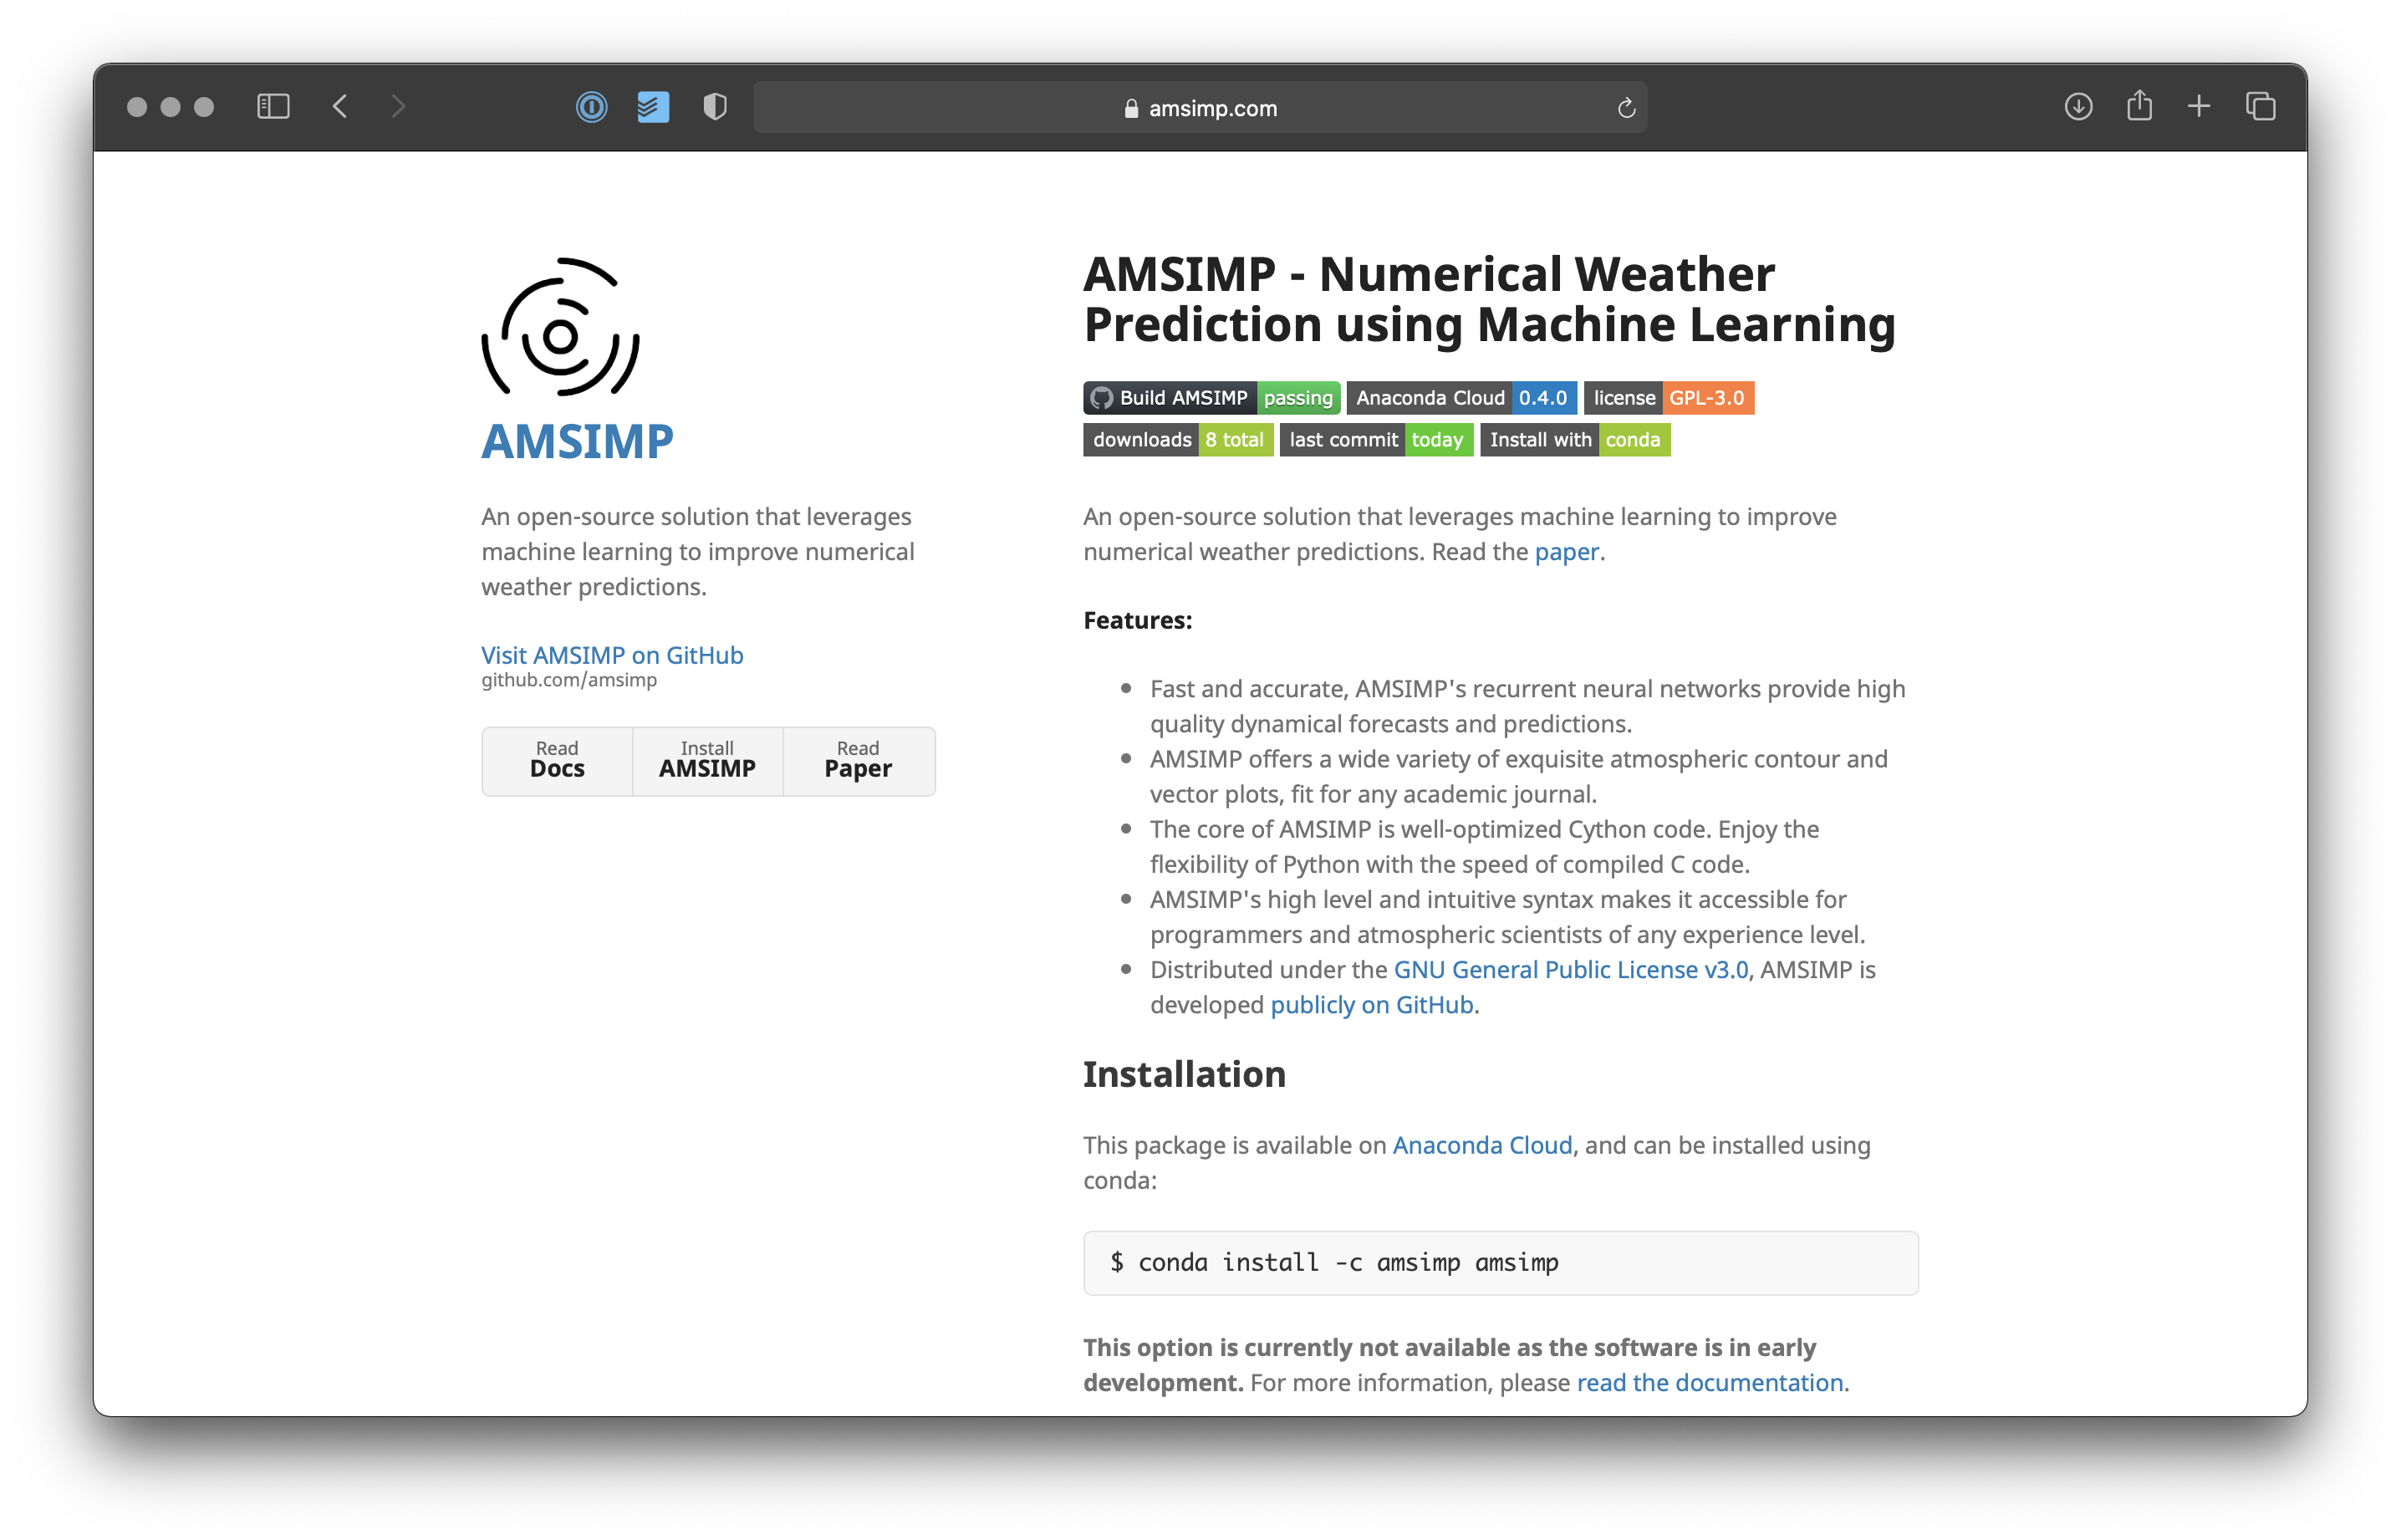
\includegraphics[width=.75\linewidth]{Images/website}
    \caption{A screenshot of the website for the software.}
    \label{website}
\end{figure}

\section{Organisation of this Work}
The work contained in this project book is broken down into a number of different chapters:

\begin{itemize}
    \item Chapter \ref{architecture_chapter} discusses the various neural network architecture under consideration and the current implementation within the software.
    \item Chapter \ref{implementation_chapter} discusses some of the decisions made on the software development side of the project, such as, choosing an appropriate programming language for the task. 
    \item Chapter \ref{benchmarking_chapter} outlines the software benchmarking experiments to be carried out on the software.
    \item Chapter \ref{results_chapter} contains the results of the benchmarking described in the previous chapter.
    \item Chapter \ref{conclusion_chapter} reviews the results and outcomes of the project, discusses the limitations of the software, and lays out a road-map for the continued development and enhancement of the software. 
\end{itemize}
